\documentclass[11pt]{article}
\usepackage[letterpaper,margin=0.85in]{geometry}
\usepackage{amsmath}
\usepackage{enumitem}
\usepackage{titlesec}
\usepackage{graphicx}
\usepackage[hidelinks]{hyperref}
\setlist{nosep,leftmargin=1.2em}
\titleformat{\section}{\normalsize\bfseries}{\thesection}{0.5em}{}
\titlespacing*{\section}{0pt}{8pt}{3pt}
\setlength{\parskip}{4pt}
\setlength{\parindent}{0pt}
\setlength{\textfloatsep}{8pt}
\usepackage{caption}
\captionsetup{font=small,labelfont=bf}

\title{\vspace{-2.4em}\textbf{Rollin' Down the Biggest Hill}\\
\large CS 351 Analysis of Algorithms, Project Checkpoint}
\author{The \textsc{wheel} Ones: Conor Vahey, Felicity Chin, Oscar Yaun\\
\small Repository: \url{https://github.com/qcnr/Heely-Analysis}\quad
Analysis draft: separate PDF (\texttt{report/analysis\_draft.pdf})}
\date{\vspace{-2.6em}}

\begin{document}
\maketitle

\section{(a) The question, and what changed since the proposal}

\textbf{Question.} Given a map with elevation, find the best route between two points for someone on Heelys, and compare how much work Dijkstra's algorithm and ALT (A*, Landmarks, Triangle inequality) do to find it. The map is a directed graph. Rolling downhill costs $0$, and a flat or uphill stretch costs $1$ (one ``push''). The best route is the one with the fewest pushes. Both algorithms must return a route with that cost, and we compare their running times.

\textbf{Changes, and why.}
\begin{enumerate}
\item \textit{Objective: from ``highest downhill ratio'' to ``fewest pushes.''} A ratio is not a sum of edge costs, so it is not a shortest-path problem, and neither algorithm can find it directly. ``Fewest pushes'' keeps the same idea (roll, don't push) and is a sum of non-negative edge costs, which is what both algorithms need.
\item \textit{Weights flipped.} The proposal gave downhill a weight of $1$ and everything else $0$. We use downhill $=0$ and flat/uphill $=1$, so that the shortest path is the route we actually want.
\item \textit{Schedule.} The proposal had both algorithms started by Nov 4. Dijkstra, the test grids, the correctness checks and the timing code are done; ALT is not started yet. Section~(d) has the updated plan.
\end{enumerate}

\section{(b) What is implemented, and how we know it is correct}

All code is Python. Implemented:
\begin{itemize}
\item \texttt{heely/graph.py}: generates an $n\times n$ grid with random hills, with edge costs as above. Seeded, so each grid can be rebuilt exactly.
\item \texttt{heely/dijkstra.py}: our own Dijkstra with a binary heap, stopping when the goal is reached. Returns the route, its cost, and how many nodes it settled.
\item \texttt{heely/experiment.py} and \texttt{heely/plot.py}: timing code and the plot in Section~(c).
\end{itemize}

\textbf{Evidence of correctness} (\texttt{python -m pytest -q}, 10 tests; brute force lives in the tests, not in the algorithm code):
\begin{itemize}
\item \textit{Hand-checked world.} A $3\times3$ hill where the right answers can be worked out by hand (peak to any corner is $0$ pushes, corner to peak is $2$).
\item \textit{Brute force on small grids.} On five grids from $2\times2$ to $4\times4$, for all $690$ start/goal pairs, Dijkstra's cost matches the cheapest of every possible path.
\item \textit{Larger grids.} Brute force is too slow past $4\times4$, so on grids up to $60\times60$ we check Dijkstra's distances directly: the start has distance $0$, no edge offers a shortcut ($d[v]\le d[u]+w(u,v)$ for every edge), and every node's distance is reached by a real edge from its parent. Distances that pass these checks are the true shortest distances (a standard check; see CLRS Chapter~22), so no second algorithm is needed. All $9$ full runs pass.
\item \textit{Routes, not just costs.} Every returned route is checked step by step: each step is a real edge, no node repeats, and the pushes add up to the reported cost.
\end{itemize}

\section{(c) Preliminary results}

\begin{figure}[h]
\centering
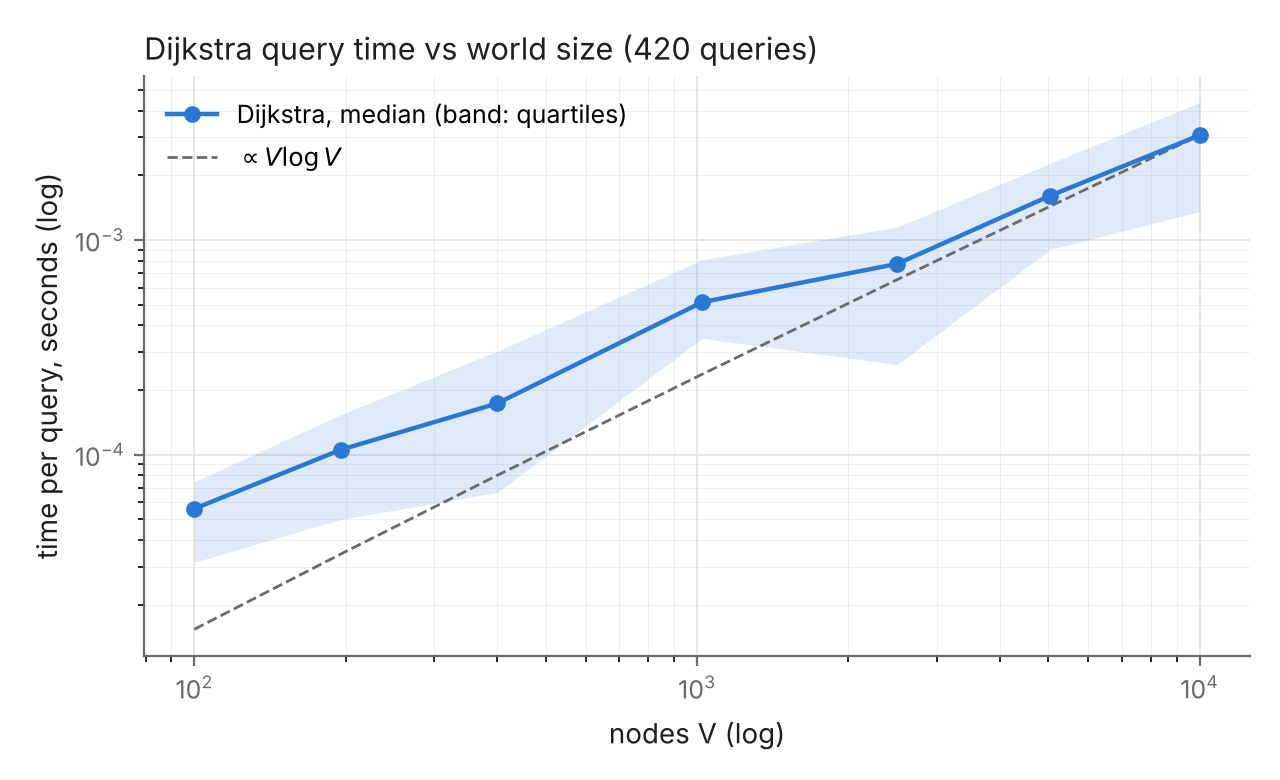
\includegraphics[width=0.78\textwidth]{../results/preliminary_plot.png}
\caption{Dijkstra query time against number of nodes $V$, log-log. Three random grids at each of seven sizes ($10\times10$ to $100\times100$, so $100$ to $10{,}000$ nodes), $20$ random start/goal queries per grid, $420$ queries total. Line: median. Band: 25th to 75th percentile. Dashed line: $V\log V$, scaled to the last point.}
\end{figure}

\begin{itemize}
\item Query time grows in line with the $V\log V$ reference, as the analysis predicts: from a mean of $0.05$ ms at $100$ nodes to $3.0$ ms at $10{,}000$ nodes.
\item On average Dijkstra settles about half of all nodes before reaching the goal ($44\%$ to $54\%$ across the sizes), because it spreads out evenly in every direction instead of heading toward the goal. This is the number ALT should reduce, and it is what we will compare.
\item The spread is wide because the cost of a query depends a lot on where the start and goal are relative to the hills.
\end{itemize}

\section{(d) What remains, and the schedule}

\begin{itemize}
\item \textbf{By Nov 16.} Implement ALT (choose landmarks, precompute distances to and from them, run A*), test that it gives the same cost as Dijkstra on every query, and add it to the timing code so both run on the same grids and queries.
\item \textbf{By Nov 20.} Run the full comparison and make the final plots. Write the ALT correctness and running-time analysis. Try the real-world CoMaps/GPX data; if it is not working by Nov 20, it becomes a future-work note, as planned in the proposal.
\item \textbf{By Nov 30.} Write the final report and presentation, then practice the presentation.
\end{itemize}

\section{(e) Contributions}

[\textit{Team: edit this before submitting so it says what each person actually did.}] Conor built the grid generator, Dijkstra, the tests and timing code, and drafted the analysis and this report. Felicity and Oscar are implementing ALT and will write its analysis.

\end{document}
